\documentclass[10pt]{article}
\usepackage[margin=0.7in]{geometry}
\usepackage[T1]{fontenc}
\usepackage{lmodern,amsmath,graphicx,booktabs,hyperref}
\hypersetup{colorlinks=true,urlcolor=blue}
\setlength{\parindent}{0pt}\setlength{\parskip}{5pt}\setlength{\emergencystretch}{3em}
\begin{document}
{\Large\bfseries Finite precision at the contraction root}

23 November 2026. Producer observations, PCC unverified. Formal claim
\texttt{759751}; native controls \texttt{4b3d64}. Local execution; no S3.

The exact Nat source expression now has a finite root envelope. Put
$D=2^{2u-i}$ and let $P$ denote
\[
 p+8\left\lfloor\frac{3M+u-1}{u}\right\rfloor D+8M(2u+1).
\]
For $p\le M$, $32u\le M$ and $i<u$, the shared Lean theorem proves
$Pu\le35MD$. The actual root length/array guard
$2^{2u}64^{4u}=2^{26u}\le M$ supplies $32u\le M$.
No inherited-history or asymptotic absorption assumption is used for this root.

\textbf{Proof.} The active valuation gives $D\ge2^{u+1}$.
Finite induction gives $4u\le2^{u+1}$ and
$16u(2u+1)\le21\cdot2^{u+1}$. Floor division gives
$u\lfloor(3M+u-1)/u\rfloor\le3M+u$.
The three terms of $4Pu$ are bounded by $MD$, $97MD$ and $42MD$;
addition and cancellation give35. The shared owner is crypto-lean,
commit \texttt{1c57c092460b}; the study only instantiates its laws.

\begin{center}
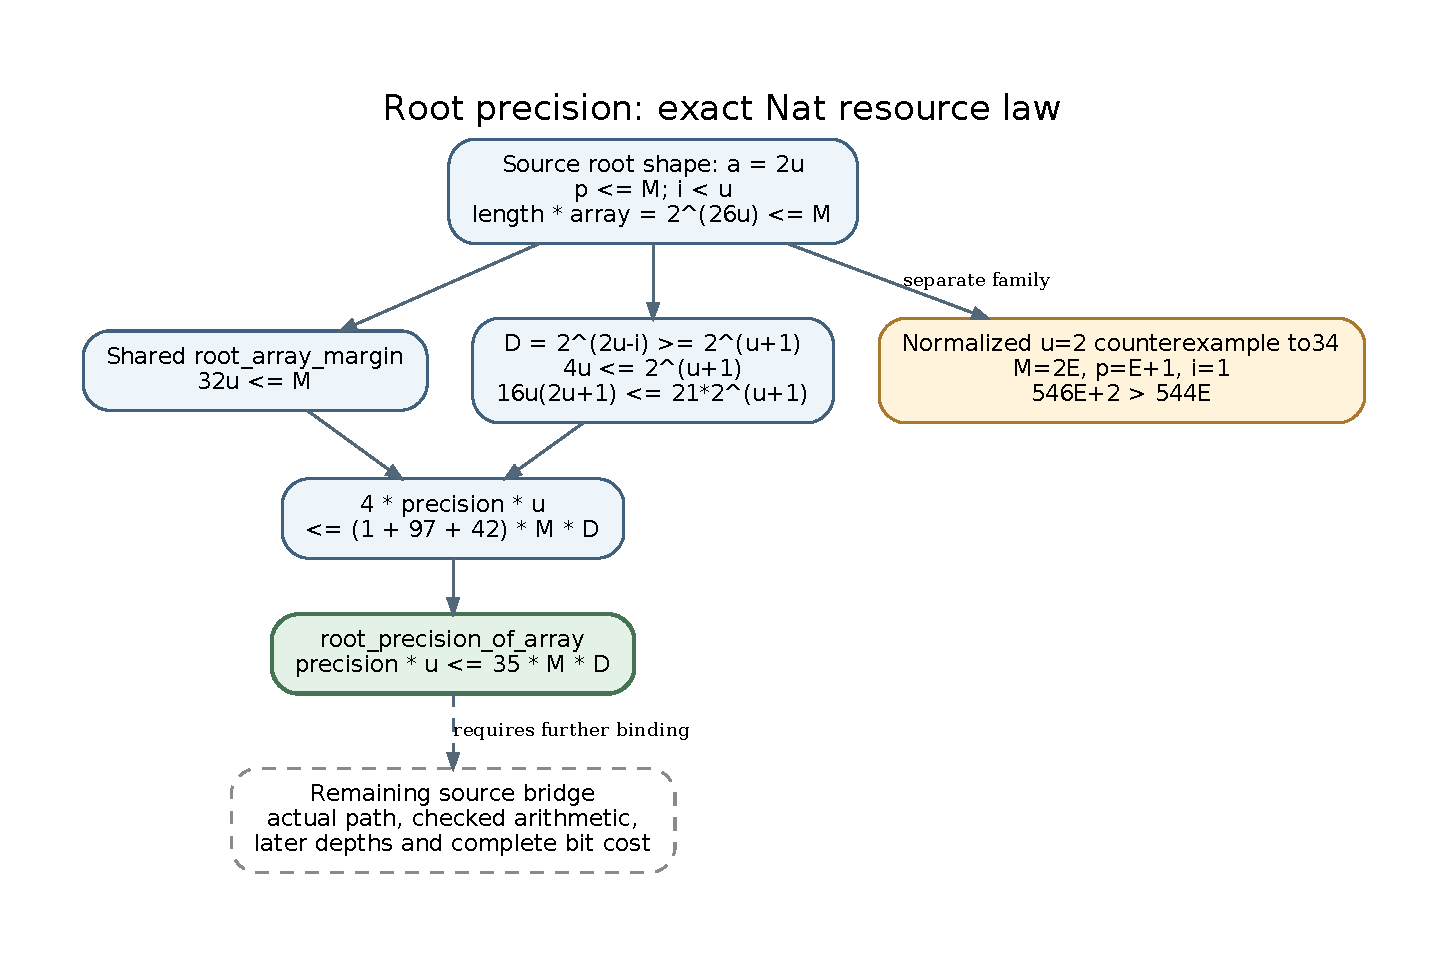
\includegraphics[width=0.91\linewidth,height=3.65in,keepaspectratio]{proof-map.pdf}
\end{center}

\textbf{Why34 needs its extra premises.} With $M=2E,p=E+1,u=2,a=4,i=1$,
\[
 2P=546E+2>544E=34MD.
\]
For the weaker margin domain take $E\ge32$; the full array guard needs
$E\ge2^{51}$. The prior conditional34 and finite-history81 laws are unchanged.
The primary AppendixD.11 is an asymptotic Big-O result, not an explicit universal34
assertion. The next source obligation is actual path, checked arithmetic and
complete bit-cost binding, including later depths and rational widths.

\newpage
{\large\bfseries Controls, evidence and scope}

\begin{tabular}{p{0.48\linewidth}p{0.46\linewidth}}
\toprule
Check & Observed outcome\\\midrule
Shared / study formal declarations &5 /7 compile; unchanged axiom gates pass\\
Explicit axiom queries &12, standard foundations only\\
Official fresh kernel replay &\texttt{leanchecker --fresh RootControls}, exit0\\
PCC statement binding / proof gates &Local verifier pass; signed standing unverified\\
Translated exact Setup witness &All21 scalar checks pass\\
Single-field source corruptions &7/7 rejected\\
Weaker margin-domain sweep &29,952/29,952 satisfy35;12 exact rational maxima retained\\
Source and copied binary hashes &All pre/post identities unchanged\\
\bottomrule
\end{tabular}

\textbf{Native positive witness.} Rust1.99.1 BigUint uses
$M=s=2^{262150}$, $p=M/2+1$, degree2, $\lambda=262150$,
$\lfloor\sqrt\lambda\rfloor=512$, $\delta=2^{235935}$,
$u=2,a=4,L=16$, array$=2^{48}$ and $t=2$.
The exact certificate $\delta^{10}=s^9$ fixes the root rounding;
leaf$=2^{262141}<M$. Degree, length/array, active valuation, source ceiling,
normalized precision,35 and34 checks all pass. Changing lambda,u,delta,sqrt,
degree,valuation or array individually is rejected.

\textbf{Premise deletion.} The native controls explicitly check all remaining
premises and failure of the omitted one. These examples concern the weaker
scalar domain; the margin deletion also drops the stronger array guard.

\begin{center}\begin{tabular}{lrr}
\toprule
Omitted premise & Actual precision$\times u$ &35-envelope\\\midrule
$p\le M$ &4864&4480\\
$32u\le M$ &886&840\\
$i<u$ &2336&2240\\\bottomrule
\end{tabular}\end{center}
At $E=32$, the abstract34 counterexample is17474$>$17408;35 gives17920.

\textbf{Exact scope.} The witness translates unbounded integer scalar guards;
it allocates no graph and is not a production Setup call. Current64-bit usize
has $\lambda\le64$, hence root\_u0. The huge witness's $u=2$ does not satisfy
the paper's sufficiently-large consequence $u\ge\lambda^{4/5}$ and is not a
counterexample to the paper. The29,952 small cases use $u=1..12$,
$M=32u..32u+127$, $p\in\{0,\lfloor M/2\rfloor+1,M\}$ and $i=0..u-1$;
they are controls for the universal Lean theorem, not its proof.

\textbf{Retained failures and limits.} Attempts01/01b failed compiler-root/name
setup;02 failed proof normalization/API use;03 failed import layout.04/04b hit
the unchanged15,032,385,536-byte whole-cgroup stop. Lossless cache/readback
archives were compared before space reclamation;04c passed. One worker,
600s phase ceilings and60s native ceiling stayed fixed. No theorem assumption,
toolchain or limit was relaxed. All old CPU records and34/81 proofs are intact.

\textbf{Review and publication.} Written same-root-team reviews are source/math
checks, not independent execution. Standard foundations are propext/Quot.sound,
with Classical.choice in one consumer proof and none in three literal controls.
No holes, custom axioms or native\_decide occur. The fresh checker is Lean's own
kernel. Current-main PCC ledger prefix diverges at1564; both histories remain,
so signed standing/merge integration is open. No canonical runtime chart changes.

\small Sources: pinned AppendixD.11 (OpenAI/math42907c9e), recursive.rs at
crypto d562832c, shared core3e47fb77 and root1c57c092. KB unavailable127;
bounded exact-source fallback supplies no novelty clearance. Full receipts,
source hashes, raw native output, proof map and failed attempts accompany this report.\par
\url{https://github.com/isogeny-labs/crypto/pull/4996}\par
\url{https://github.com/aburan28/crypto-lean/pull/35}
\end{document}
